\documentclass[10pt]{article}

\usepackage[italian]{babel}
\usepackage[utf8]{inputenc}
\usepackage[margin=1.0in]{geometry}

\usepackage{amsmath,amsfonts,amssymb,mathtools, ulem, booktabs,subcaption, float}
\usepackage{graphicx}
\usepackage{xcolor}
\usepackage{multirow}
\graphicspath{ {./images/} }

\title{Reti: Esercizi}
\author{Aymane Chabbaki}
\date{III semestre 2019/2020}
\begin{document}
	\maketitle
	\tableofcontents
	\newpage
	
\section{Routing: Link State (OSPF)}
	\subsection{Esercizio 1}
	Usando gli algoritmi propri di OSPF, ed assumendo che i costi siano già stati distribuiti, si calcoli la tabella di instradamento del nodo A.
	\begin{figure}[h]
	\centering
	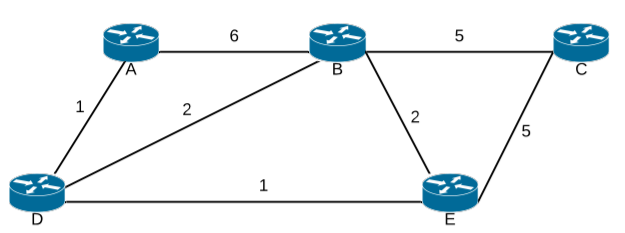
\includegraphics[width=13cm]{es1}
	\end{figure}
	\begin{center}
	\textbf{A}
 		\begin{tabular}{||c c c c c c||} 
 			\hline
 			Step & N' & $D(B)$ & $D(D)$ & $D(E)$ & $D(C)$ \\[0.5ex] 
 			\hline\hline
 			0 & $A$ & $6,A$ & $\color{red} 1,A$ & $\infty$ & $\infty$ \\ 
 			\hline
			1 & $A,D$ & $3,D$ &   & $\color{red}2,D$ & $\infty$ \\
 			\hline
 			2 & $A,D,E$ & $\color{red}3,D$ &   &   & $7,E$ \\
 			\hline
			3 & $A,D,E,B$ &   &   &   & $\color{red}7,E$\\[0.5ex] 
 			\hline
		\end{tabular}
		\quad
		\begin{tabular}{||c || c || c||}
			\hline
 			Destination & Cost & Next Hop\\ [0.5ex] 
 			\hline\hline
			$A$ & $0$ & $-$\\
			$B$ & $3$ & $D$\\
 			$C$ & $7$ & $D$\\
			$D$ & $1$ & $D$\\
			$E$ & $2$ & $D$\\[0.5ex] 
			\hline
		\end{tabular}
	\end{center}
	
	\subsection{Esercizio 2}
	Usando gli algoritmi propri di OSPF, ed assumendo che i costi siano già stati distribuiti, si calcoli la tabella di instradamento del nodo A.
	\begin{figure}[h]
	\centering
	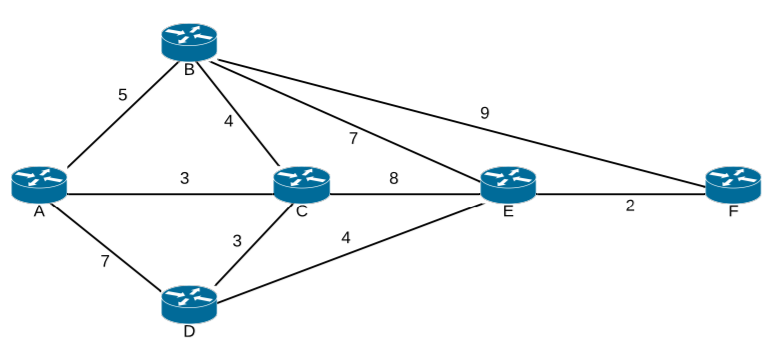
\includegraphics[width=13cm]{es2}
	\end{figure}
	\begin{center}
	\textbf{A}
 		\begin{tabular}{||c c c c c c c||} 
 			\hline
 			Step & N' & $D(B)$ & $D(C)$ & $D(D)$ & $D(E)$ & $D(F)$ \\[0.5ex] 
 			\hline\hline
 			0 & $A$ & $5,A$ & $\color{red} 3,A$ & $7,A$ & $\infty$ & $\infty$ \\ 
 			\hline
 			1 & $A,C$ & $\color{red} 5,A$ & & $6,C$ & $11,C$ & $\infty$ \\ 
 			\hline
 			2 & $A,C,B$ & & & $\color{red} 6,C$ & $11,C$ & $14,B$ \\
 			\hline
 			3 & $A,C,B,D$ & & & & $\color{red} 10,D$ & $14,B$ \\
 			\hline
 			4 & $A,C,B,D,E$ & & & & & $\color{red} 12,E$ \\[0.5ex] 
 			\hline
		\end{tabular}
		\quad
		\begin{tabular}{||c || c || c||}
			\hline
 			Destination & Cost & Next Hop\\[0.5ex] 
 			\hline\hline
			$A$ & $0$ & $-$\\
			$B$ & $5$ & $B$\\
 			$C$ & $3$ & $C$\\
			$D$ & $6$ & $C$\\
			$E$ & $10$ & $C$\\
			$F$ & $12$ & $C$\\[0.5ex] 
			\hline
		\end{tabular}
	\end{center}
	
	\subsection{Esercizio 3}
	Usando gli algoritmi propri di OSPF, ed assumendo che i costi siano già stati distribuiti, si calcoli la tabella di instradamento del nodo A.
	\begin{figure}[h]
	\centering
	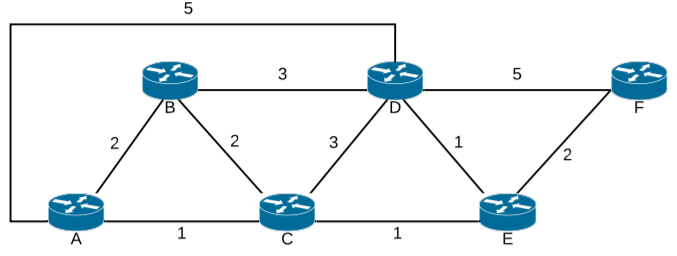
\includegraphics[width=13cm]{es3}
	\end{figure}
	\begin{center}
	\textbf{A}
 		\begin{tabular}{||c c c c c c c||} 
 			\hline
 			Step & N' & $D(B)$ & $D(C)$ & $D(D)$ & $D(E)$ & $D(F)$ \\[0.5ex] 
 			\hline\hline
 			0 & $A$ & $2,A$ & $\color{red} 1,A$ & $5,A$ & $\infty$ & $\infty$ \\
 			\hline
 			1 & $A,C$ & $2,A$ & & $4,C$ & $\color{red} 2,C$ & $\infty$ \\
 			\hline
 			2 & $A,C,E$ & $\color{red} 2,A$ & & $3,E$ & & $4,E$ \\
 			\hline
 			3 & $A,C,E,B$ & & & $\color{red} 3,E$ & & $4,E$ \\
 			\hline
 			4 & $A,C,E,B,D$ & & & & & $\color{red} 4,E$ \\[0.5ex] 
 			\hline
		\end{tabular}
		\quad
		\begin{tabular}{||c || c || c||}
			\hline
 			Destination & Cost & Next Hop\\[0.5ex] 
 			\hline\hline
			$A$ & $0$ & $-$\\
			$B$ & $2$ & $B$\\
 			$C$ & $1$ & $C$\\
			$D$ & $3$ & $C$\\
			$E$ & $2$ & $C$\\
			$F$ & $4$ & $C$\\[0.5ex] 
			\hline
		\end{tabular}
	\end{center}
	
	\subsection{Esercizio 4}
	Usando gli algoritmi propri di OSPF, ed assumendo che i costi siano già stati distribuiti, si calcoli la tabella di instradamento del nodo E.
	\begin{figure}[h]
	\centering
	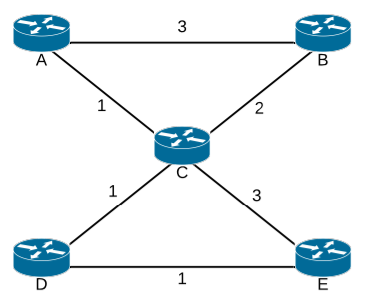
\includegraphics[width=6cm]{es5}
	\end{figure}
	\begin{center}
	\textbf{E}
 		\begin{tabular}{||c c c c c c||} 
 			\hline
 			Step & N' & $D(A)$ & $D(B)$ & $D(C)$ & $D(D)$ \\[0.5ex] 
 			\hline\hline
 			0 & $E$ & $\infty$ & $\infty$ & $3,E$ & $\color{red} 1,E$ \\
 			\hline
 			1 & $E,D$ & $\infty$ & $\infty$ & $\color{red} 2,E$ & \\
 			\hline
 			2 & $E,D,C$ & $\color{red} 3,C$ & $4,C$ &  & \\
 			\hline
 			3 & $E,D,C,A$ & & $\color{red} 4,C$ & & \\[0.5ex] 
 			\hline
		\end{tabular}
		\quad
		\begin{tabular}{||c || c || c||}
			\hline
 			Destination & Cost & Next Hop\\[0.5ex] 
 			\hline\hline
			$A$ & $3$ & $D$\\
			$B$ & $4$ & $D$\\
 			$C$ & $2$ & $D$\\
			$D$ & $1$ & $D$\\
			$E$ & $0$ & $-$\\[0.5ex] 
			\hline
		\end{tabular}
	\end{center}
	\newpage
	\subsection{Esercizio 5}
	Usando gli algoritmi propri di OSPF, ed assumendo che i costi siano già stati distribuiti, si calcoli la tabella di instradamento dei nodi ${B,D,F}$.
	\begin{figure}[h]
	\centering
	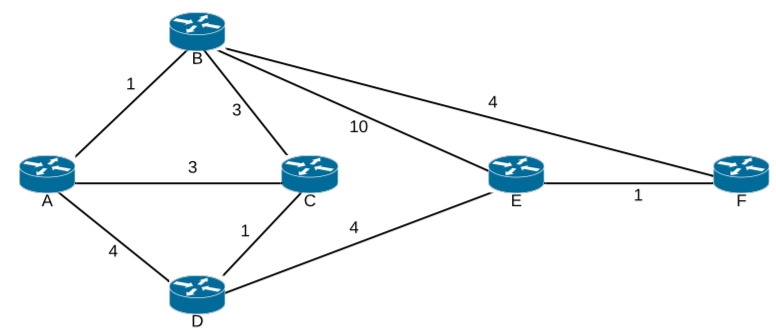
\includegraphics[width=13cm]{es4}
	\end{figure}
	\begin{center}
	 	\textbf{B}
 		\begin{tabular}{||c c c c c c c||} 
 			\hline
 			Step & N' & $D(A)$ & $D(C)$ & $D(D)$ & $D(E)$ & $D(F)$ \\[0.5ex] 
 			\hline\hline
 			0 & $B$ & $\color{red} 1,B$ & $3,B$ & $\infty$ & $10,B$ & $4,B$ \\
 			\hline
 			1 & $B,A$ &  & $\color{red} 3,B$ & $5,A$ & $10,B$ & $4,B$ \\
 			\hline
 			2 & $B,A,C$ & & & $\color{red} 4,C$ & $10,B$ & $4,B$ \\
 			\hline
 			3 & $B,A,C,D$ & & & & $8,D$ & $\color{red} 4,B$ \\
 			\hline
 			4 & $B,A,C,D,F$ & & & & $\color{red} 5,F$ & \\[0.5ex]  
 			\hline
		\end{tabular}
		\quad
		\begin{tabular}{||c || c || c||}
			\hline
 			Destination & Cost & Next Hop\\[0.5ex] 
 			\hline\hline
			$A$ & $1$ & $A$\\
			$B$ & $0$ & $-$\\
 			$C$ & $3$ & $C$\\
			$D$ & $4$ & $C$\\
			$E$ & $5$ & $F$\\
			$F$ & $4$ & $F$\\[0.5ex]
			\hline
		\end{tabular}
	\end{center}
	
	\begin{center}
	 	\textbf{D}
 		\begin{tabular}{||c c c c c c c||} 
 			\hline
 			Step & N' & $D(A)$ & $D(B)$ & $D(C)$ & $D(E)$ & $D(F)$ \\[0.5ex] 
 			\hline\hline
 			0 & $D$ & $4,D$ & $\infty$ & $\color{red} 1,D$ & $4,D$ & $\infty$ \\
 			\hline
 			1 & $D,C$ & $\color{red} 4,D$ & $4,C$ & & $4,D$ & $\infty$ \\
 			\hline
 			2 & $D,C,A$ & & $\color{red} 4,C$ & & $4,D$ & $\infty$ \\
 			\hline
 			3 & $D,C,A,B$ & & & & $\color{red} 4,D$ & $8,B$ \\
 			\hline
 			4 & $D,C,A,B,E$ & & & & & $\color{red} 5,E$ \\[0.5ex]  
 			\hline
		\end{tabular}
		\quad
		\begin{tabular}{||c || c || c||}
			\hline
 			Destination & Cost & Next Hop\\[0.5ex] 
 			\hline\hline
			$A$ & $4$ & $A$\\
			$B$ & $4$ & $C$\\
 			$C$ & $1$ & $C$\\
			$D$ & $0$ & $-$\\
			$E$ & $4$ & $E$\\
			$F$ & $5$ & $E$\\[0.5ex]
			\hline
		\end{tabular}
	\end{center}
	
	\begin{center}
	 	\textbf{F}
 		\begin{tabular}{||c c c c c c c||} 
 			\hline
 			Step & N' & $D(A)$ & $D(B)$ & $D(C)$ & $D(E)$ & $D(F)$ \\[0.5ex] 
 			\hline\hline
 			0 & $F$ & $\infty$ & $4,F$ & $\infty$ & $\infty$ & $\color{red} 1,F$ \\
 			\hline
 			1 & $F,E$ & $\infty$ & $\color{red} 4,F$ & $\infty$ & $5,E$  & \\
 			\hline
 			2 & $F,E,B$ & $\color{red} 5,B$ & & $7,B$ & $5,E$ & \\
 			\hline
 			3 & $F,E,B,A$ & & & $7,B$ & $\color{red} 5,E$ & \\
 			\hline
 			4 & $F,E,B,A,D$ & & & $\color{red} 6,D$ & &\\[0.5ex]  
 			\hline
		\end{tabular}
		\quad
		\begin{tabular}{||c || c || c||}
			\hline
 			Destination & Cost & Next Hop\\[0.5ex] 
 			\hline\hline
			$A$ & $5$ & $B$\\
			$B$ & $4$ & $B$\\
 			$C$ & $6$ & $E$\\
			$D$ & $5$ & $E$\\
			$E$ & $1$ & $E$\\
			$F$ & $0$ & $-$\\[0.5ex]
			\hline
		\end{tabular}
	\end{center}
	
	\newpage
	
	\subsection{Esercizio 6}
	Usando gli algoritmi propri di OSPF, ed assumendo che i costi siano già stati distribuiti, si calcoli la tabella di instradamento dei nodi ${B,C,E,F}$.
	\begin{figure}[h]
	\centering
	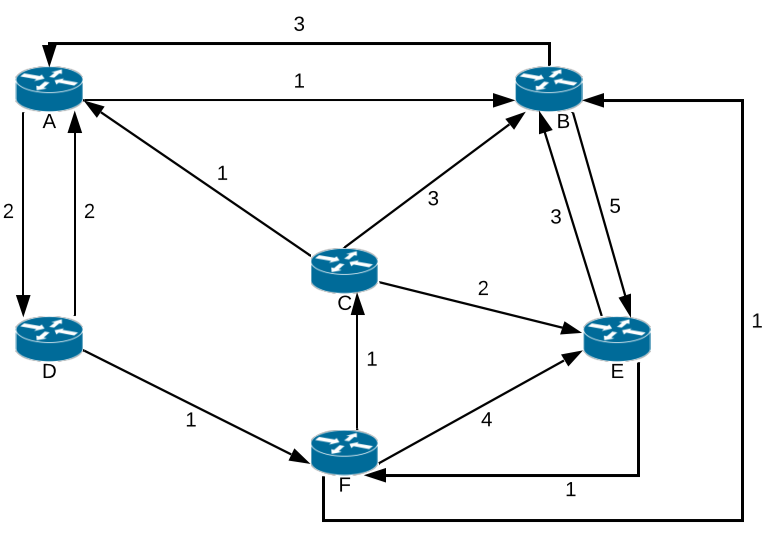
\includegraphics[width=10cm]{es6}
	\end{figure}
	\begin{center}
	 	\textbf{B}
 		\begin{tabular}{||c c c c c c c||} 
 			\hline
 			Step & N' & $D(A)$ & $D(C)$ & $D(D)$ & $D(E)$ & $D(F)$ \\[0.5ex] 
 			\hline\hline
 			0 & $A$ & $\color{red} 3,B$ & $\infty$ & $\infty$ & $5,B$ & $\infty$ \\
 			\hline
 			1 & $B,A$ & & $\infty$ & $\color{red} 5,A$ & $5,B$ & $\infty$ \\
 			\hline
 			2 & $B,A,D$ & & $\infty$ & & $\color{red} 5,B$ & $6,D$ \\
 			\hline
 			3 & $B,A,D,E$ & & $\infty$ & & & $\color{red} 6,D$ \\
 			\hline
 			4 & $B,A,D,E,F$ & & $\color{red} 7,F$ & & & \\
			\hline
		\end{tabular}
		\quad
		\begin{tabular}{||c || c || c||}
			\hline
 			Destination & Cost & Next Hop\\[0.5ex] 
 			\hline\hline
			$A$ & $3$ & $A$\\
			$B$ & $0$ & $-$\\
 			$C$ & $7$ & $A$\\
			$D$ & $5$ & $A$\\
			$E$ & $5$ & $B$\\
			$F$ & $6$ & $A$\\[0.5ex]
			\hline
		\end{tabular}
	\end{center}
	
	\begin{center}
	 	\textbf{C} \quad
 		\begin{tabular}{||c c c c c c c||} 
 			\hline
 			Step & N' & $D(A)$ & $D(B)$ & $D(D)$ & $D(E)$ & $D(F)$ \\[0.5ex] 
 			\hline\hline
 			0 & $C$ & $\color{red} 1,C$ & $3,C$ & $\infty$ & $2,C$ & $\infty$ \\
 			\hline
 			1 & $C,A$ & & $\color{red} 2,A$ & $3,A$ & $2,C$ & $\infty$ \\
 			\hline
 			2 & $C,A,B$ & & & $3,A$ & $\color{red} 2,C$ & $\infty$ \\
 			\hline
 			3 & $C,A,B,E$ & & & $\color{red} 3,A$ & & $3,E$ \\
 			\hline
 			4 & $C,A,B,E$ & & & & & $\color{red} 3,E$ \\
 			\hline
		\end{tabular}
		\quad
		\begin{tabular}{||c || c || c||}
			\hline
 			Destination & Cost & Next Hop\\[0.5ex] 
 			\hline\hline
			$A$ & $1$ & $A$\\
			$B$ & $2$ & $A$\\
 			$C$ & $0$ & $-$\\
			$D$ & $3$ & $A$\\
			$E$ & $2$ & $E$\\
			$F$ & $3$ & $E$\\[0.5ex]
			\hline
		\end{tabular}
	\end{center}	
	
	\begin{center}
	 	\textbf{E}
 		\begin{tabular}{||c c c c c c c||} 
 			\hline
 			Step & N' & $D(A)$ & $D(B)$ & $D(C)$ & $D(D)$ & $D(F)$ \\[0.5ex] 
 			\hline\hline
 			0 & $E$ & $\infty$ & $3,E$ & $\infty$ & $\infty$ & $\color{red} 1,E$ \\
 			\hline
 			1 & $E,F$ & $\infty$ & $\color{red} 2,F$ & $2,F$ & $\infty$ & \\
 			\hline
 			2 & $E,F,B$ & $5,B$ & & $\color{red} 2,F$ & $\infty$ & \\
 			\hline
 			3 & $E,F,B,C$ & $\color{red} 3,C$ & & & $\infty$ & \\
 			\hline
 			4 & $E,F,B,C,A$ & & & & $\color{red} 5,A$ & \\[0.5ex]  
 			\hline
		\end{tabular}
		\quad
		\begin{tabular}{||c || c || c||}
			\hline
 			Destination & Cost & Next Hop\\[0.5ex] 
 			\hline\hline
			$A$ & $3$ & $F$\\
			$B$ & $2$ & $F$\\
 			$C$ & $2$ & $F$\\
			$D$ & $5$ & $F$\\
			$E$ & $0$ & $-$\\
			$F$ & $1$ & $F$\\[0.5ex]
			\hline
		\end{tabular}
	\end{center}
	
	\begin{center}
	 	\textbf{F}
 		\begin{tabular}{||c c c c c c c||} 
 			\hline
 			Step & N' & $D(A)$ & $D(B)$ & $D(C)$ & $D(D)$ & $D(E)$ \\[0.5ex] 
 			\hline\hline
 			0 & $F$ & $\infty$ & $\color{red} 1,F$ & $1,F$ & $\infty$ & $4,F$ \\
 			\hline
 			1 & $F,B$ & $4,B$ & & $\color{red} 1,F$ & $\infty$ & $4,F$ \\
 			\hline
 			2 & $F,B,C$& $\color{red} 2,C$ & & & $\infty$ & $3,C$ \\
 			\hline
 			3 & $F,B,C,A$ & & & & $4,A$ & $\color{red} 3,C$ \\
 			\hline
 			4 & $F,B,C,A,E$ & & & & $\color{red} 4,A$ & \\[0.5ex]  
 			\hline
		\end{tabular}
		\quad
		\begin{tabular}{||c || c || c||}
			\hline
 			Destination & Cost & Next Hop\\[0.5ex] 
 			\hline\hline
			$A$ & $2$ & $C$\\
			$B$ & $1$ & $B$\\
 			$C$ & $1$ & $C$\\
			$D$ & $4$ & $C$\\
			$E$ & $3$ & $C$\\
			$F$ & $0$ & $-$\\[0.5ex]
			\hline
		\end{tabular}
	\end{center}

	\subsection{Esercizio 7}
	Usando gli algoritmi propri di OSPF, ed assumendo che i costi siano già stati distribuiti, si calcoli la tabella di instradamento dei nodi ${A,G}$.
	\begin{figure}[h]
	\centering
	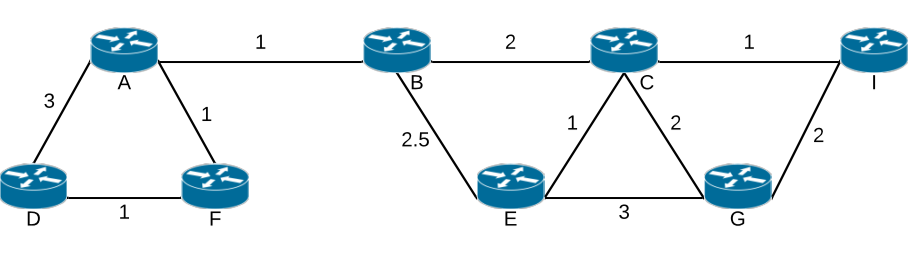
\includegraphics[width=13cm]{es7}
	\end{figure}
	\begin{center}
	\textbf{A}
 		\begin{tabular}{||c c c c c c c c c||} 
 			\hline
 			Step & N' & $D(B)$ & $D(C)$ & $D(D)$ & $D(E)$ & $D(F)$ & $D(G)$ & $D(I)$ \\
 			\hline\hline
 			0 & $A$ & $\color{red} 1,A$ & $\infty$ & $3,A$ & $\infty$ & $1,A$ & $\infty$ & $\infty$ \\
 			\hline
 			1 & $A,B$ & & $3,B$ & $3,A$ & $3.5,B$ & $\color{red} 1,A$ & $\infty$ & $\infty$ \\
 			\hline
			2 & $A,B,F$ & & $3,B$ & $\color{red} 2,F$ & $3.5,B$ & & $\infty$ & $\infty$ \\
			\hline
			3 & $A,B,F,D$ & & $\color{red} 3,B$ & & $3.5,B$ & & $\infty$ & $\infty$ \\ 
 			\hline
			4 & $A,B,F,D,C$ & & & & $\color{red} 3.5,B$ & & $5,C$ & $4,C$ \\
			\hline
			5 & $A,B,F,D,C,E$ & & & & & & $5,C$ & $\color{red} 4,C$ \\
			\hline
			6 & $A,B,F,D,C,E,I$ & & & & & & $\color{red} 5,C$ & \\[0.5ex]
 			\hline
		\end{tabular}
	\end{center}
	\begin{center}
	\textbf{A:}
		\begin{tabular}{||c || c || c||}
			\hline
 			Destination & Cost & Next Hop\\ [0.5ex] 
 			\hline\hline
			$A$ & $0$ & $-$\\
			$B$ & $1$ & $B$\\
 			$C$ & $3$ & $B$\\
			$D$ & $2$ & $F$\\
			$E$ & $3.5$ & $B$\\
			$F$ & $1$ & $F$\\
			$G$ & $5$ & $B$\\
			$I$ & $4$ & $B$\\[0.5ex] 
			\hline
		\end{tabular}
	\end{center}	
	
	\begin{center}
	\textbf{G}
 		\begin{tabular}{||c c c c c c c c c||} 
 			\hline
 			Step & N' & $D(A)$ & $D(B)$ & $D(C)$ & $D(D)$ & $D(E)$ & $D(F)$ & $D(I)$ \\
 			\hline\hline
 			0 & $G$ & $\infty$ & $\infty$ & $\color{red} 2,G$ & $\infty$ & $3,G$ & $\infty$ & $2,G$ \\
 			\hline
 			1 & $G,C$ & $\infty$ & $4,C$ & & $\infty$ & $3,G$ & $\infty$ & $\color{red} 2,G$ \\
 			\hline
			2 & $G,C,I$ & $\infty$ & $4,C$ & & $\infty$ & $\color{red} 3,G$ & $\infty$ & \\
			\hline
			3 & $G,C,I,E$ & $\infty$ & $\color{red} 4,C$ & & $\infty$ & & $\infty$ & \\ 
 			\hline
			4 & $G,C,I,E,B$ & $\color{red} 5,B$ & & & $\infty$ & & $\infty$ & \\
			\hline
			5 & $G,C,I,E,B,A$ & & & & $8,A$ & & $\color{red} 6,A$ & \\
			\hline
			6 & $G,C,I,E,B,A,F$ & & & & $\color{red} 7,F$ & & & \\[0.5ex]
 			\hline
		\end{tabular}
	\end{center}
	\begin{center}
	\textbf{G:}
		\begin{tabular}{||c || c || c||}
			\hline
 			Destination & Cost & Next Hop\\ [0.5ex] 
 			\hline\hline
			$A$ & $5$ & $C$\\
			$B$ & $4$ & $C$\\
 			$C$ & $2$ & $C$\\
			$D$ & $7$ & $C$\\
			$E$ & $3$ & $E$\\
			$F$ & $6$ & $C$\\
			$G$ & $0$ & $-$\\
			$I$ & $2$ & $I$\\[0.5ex] 
			\hline
		\end{tabular}
	\end{center}		
	
	\subsection{Esercizio 8}
	
	Usando gli algoritmi propri di OSPF, ed assumendo che i costi siano già stati distribuiti, si calcoli la tabella di instradamento dei nodi ${A,B}$.
	\begin{figure}[h]
	\centering
	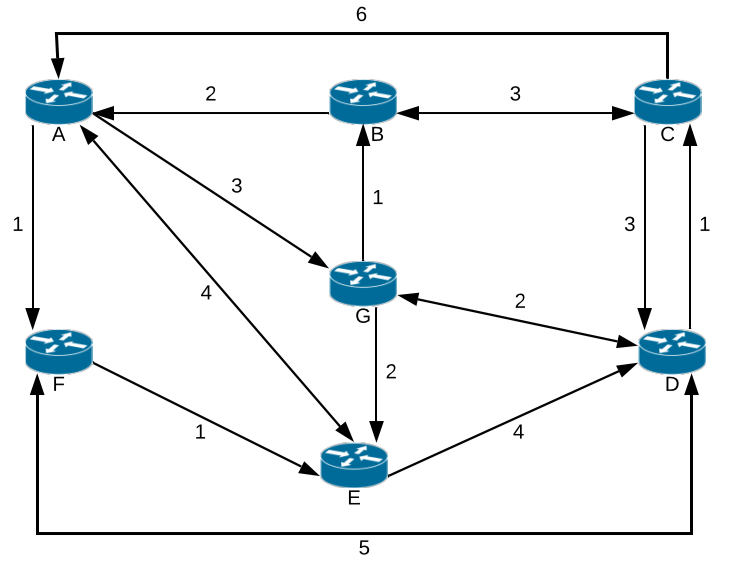
\includegraphics[width=8cm]{es8}
	\end{figure}
	\begin{center}
	\textbf{A}
 		\begin{tabular}{||c c c c c c c c||} 
 			\hline
 			Step & N' & $D(B)$ & $D(C)$ & $D(D)$ & $D(E)$ & $D(F)$ & $D(G)$ \\[0.5ex] 
 			\hline\hline
 			0 & $A$ & $\infty$ & $\infty$ & $\infty$ & $4,A$ &$\color{red} 1,A$ & $3,A$ \\
 			\hline
 			1 & $A,F$ & $\infty$ & $\infty$ & $6,F$ & $\color{red} 2,F$ & & $3,A$\\
 			\hline
 			2 & $A,F,E$ & $\infty$ & $\infty$ & $6,F$ & & & $\color{red} 3,A$ \\
 			\hline
 			3 & $A,F,E,G$ & $\color{red} 4,G$ & $\infty$ & $5,G$ & & & \\
 			\hline
 			4 & $A,F,E,G,B$ & & $7,B$ & $\color{red} 5,G$ & & & \\
 			\hline
 			5 & $A,F,E,G,B,D$ & & $\color{red} 6,D$ & & & & \\[0.5ex] 
 			\hline
		\end{tabular}
	\end{center}
	\begin{center}
	\textbf{A:}
		\begin{tabular}{||c || c || c||}
			\hline
 			Destination & Cost & Next Hop\\[0.5ex] 
 			\hline\hline
			$A$ & $0$ & $-$\\
			$B$ & $4$ & $G$\\
 			$C$ & $6$ & $G$\\
			$D$ & $5$ & $G$\\
			$E$ & $2$ & $F$\\
			$F$ & $1$ & $F$\\
			$G$ & $3$ & $G$\\[0.5ex] 
			\hline
		\end{tabular}
	\end{center}		
	
	\begin{center}
	\textbf{B}
 		\begin{tabular}{||c c c c c c c c||} 
 			\hline
 			Step & N' & $D(B)$ & $D(C)$ & $D(D)$ & $D(E)$ & $D(F)$ & $D(G)$ \\[0.5ex] 
 			\hline\hline
 			0 & $B$ & $\color{red} 2,B$ & $3,B$ & $\infty$ & $\infty$ &$\infty$ & $\infty$ \\
 			\hline
 			1 & $B,A$ & & $\color{red} 3,B$ & $\infty$ & $6,A$ & $3,A$ & $5,A$\\
 			\hline
 			2 & $B,A,C$ & & & $6,C$ & $6,A$ & $\color{red} 3,A$ & $5,A$ \\
 			\hline
 			3 & $B,A,C,F$ & & & $6,C$ & $\color{red} 4,F$ & & $5,A$ \\
 			\hline
 			4 & $B,A,C,F,E$ & & & $6,C$ & & & $\color{red} 5,A$ \\
 			\hline
 			5 & $B,A,C,F,E,G$ & & & $\color{red} 6,C$ & & & \\[0.5ex] 
 			\hline
		\end{tabular}
	\end{center}
	\begin{center}
	\textbf{B:}
		\begin{tabular}{||c || c || c||}
			\hline
 			Destination & Cost & Next Hop\\[0.5ex] 
 			\hline\hline
			$A$ & $2$ & $A$\\
			$B$ & $0$ & $-$\\
 			$C$ & $3$ & $C$\\
			$D$ & $6$ & $C$\\
			$E$ & $4$ & $A$\\
			$F$ & $3$ & $A$\\
			$G$ & $5$ & $A$\\[0.5ex] 
			\hline
		\end{tabular}
	\end{center}	
	
\newpage
\section{Routing: Distance Vector}
	\subsection{Esercizio 1}
	Usando l'algoritmo di routing di tipo Distance-vector, mostrare l'evoluzione delle tabelle di routing per ogni nodo, considerando che i DV vengono inoltrati dai router seguendo l'ordine: ${D,E,C,A,B}$.
	\begin{figure}[h!]
	\centering
	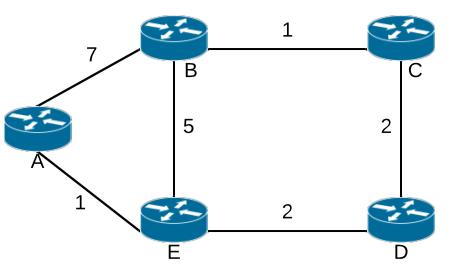
\includegraphics[width=8cm]{esercizio1}
	\end{figure}
	\newline
	Inizializzo le tabelle di routing di ogni nodo inserendo solo i nodi direttamente connessi (per semplicità includo tutte le destinazioni anche se sono ignote, queste avranno costo e NH vuoto).
	\begin{table}[h!]
		\begin{tabular}{|c||c||c|}
 			\hline
	 		\multicolumn{3}{|c|}{A} \\
 			\hline
 			Dst & Cost & NH\\
 			\hline
 			A & 0 & - \\
 			B & 7 & B \\
 			C &   &   \\
 			D &   &   \\
 			E & 1 & E \\
 			\hline
		\end{tabular}
		\begin{tabular}{|c||c||c|}
 			\hline
	 		\multicolumn{3}{|c|}{B} \\
 			\hline
 			Dst & Cost & NH\\
 			\hline
 			A & 7 & A \\
 			B & 0 & - \\
 			C & 1 & C  \\
 			D &   &   \\
 			E & 5 & E \\
 			\hline
		\end{tabular}
		\begin{tabular}{|c||c||c|}
 			\hline
	 		\multicolumn{3}{|c|}{C} \\
 			\hline
 			Dst & Cost & NH\\
 			\hline
 			A &   &   \\
 			B & 1 & B \\
 			C & 0 & - \\
 			D & 2 & D \\
 			E &   &   \\
 			\hline
		\end{tabular}
		\begin{tabular}{|c||c||c|}
 			\hline
	 		\multicolumn{3}{|c|}{D} \\
 			\hline
 			Dst & Cost & NH\\
 			\hline
 			A &   &   \\
 			B &   &   \\
 			C & 2 & C \\
 			D & 0 & - \\
 			E & 2 & E \\
 			\hline
		\end{tabular}
		\begin{tabular}{|c||c||c|}
 			\hline
	 		\multicolumn{3}{|c|}{E} \\
 			\hline
 			Dst & Cost & NH\\
 			\hline
 			A & 1 & A \\
 			B & 5 & B \\
 			C &   &   \\
 			D & 2 & D \\
 			E & 0 & - \\
 			\hline
		\end{tabular}
	\end{table}
	\newline \newline
	$D$ manda il suo DV: $\{(C,2),(E,2)\}$ a $\{E,C\}$.
	\newline
	$E$ e $C$ appena ricevono il DV, controllano se possono raggiungere una destinazione (o scoprirne una nuova) con un costo minore rispetto a quello che già conoscono.
	\newline
	$E$ per prima cosa controlla il percorso verso se stesso usando la regola dell'algoritmo: $$DV_D[E].cost + c(E,D) < R_E[E].cost?$$
	$E$ sta controllando se $2<0$, che è falso, dunque il percorso verso $D$ non viene modificato.
	\newline
	$E$ esegue la stessa procedura per $C$ e visto che $2+2 < \infty$, $E$ scopre un percorso attraverso $D$ per raggiungere $C$ (prima non conosceva $C$).
	\newline
	$C$ esegue lo stesso procedimento e viene a conoscenza del nodo $E$.
	\begin{table}[h!]
		\begin{tabular}{|c||c||c|}
 			\hline
	 		\multicolumn{3}{|c|}{A} \\
 			\hline
 			Dst & Cost & NH\\
 			\hline
 			A & 0 & - \\
 			B & 7 & B \\
 			C &   &   \\
 			D &   &   \\
 			E & 1 & E \\
 			\hline
		\end{tabular}
		\begin{tabular}{|c||c||c|}
 			\hline
	 		\multicolumn{3}{|c|}{B} \\
 			\hline
 			Dst & Cost & NH\\
 			\hline
 			A & 7 & A \\
 			B & 0 & - \\
 			C & 1 & C  \\
 			D &   &   \\
 			E & 5 & E \\
 			\hline
		\end{tabular}
		\begin{tabular}{|c||c||c|}
 			\hline
	 		\multicolumn{3}{|c|}{C} \\
 			\hline
 			Dst & Cost & NH\\
 			\hline
 			A &   &   \\
 			B & 1 & B \\
 			C & 0 & - \\
 			D & 2 & D \\
 			E & $\color{red} 4$  & $\color{red} D$ \\
 			\hline
		\end{tabular}
		\begin{tabular}{|c||c||c|}
 			\hline
	 		\multicolumn{3}{|c|}{D} \\
 			\hline
 			Dst & Cost & NH\\
 			\hline
 			A &   &   \\
 			B &   &   \\
 			C & 2 & C \\
 			D & 0 & - \\
 			E & 2 & E \\
 			\hline
		\end{tabular}
		\begin{tabular}{|c||c||c|}
 			\hline
	 		\multicolumn{3}{|c|}{E} \\
 			\hline
 			Dst & Cost & NH\\
 			\hline
 			A & 1 & A \\
 			B & 5 & B \\
 			C & $\color{red} 4$  & $\color{red} D$  \\
 			D & 2 & D \\
 			E & 0 & - \\
 			\hline
		\end{tabular}
	\end{table}
	\newline \newline \newline \newline
	$E$ manda il suo DV: $\{(A,1),(B,5),(4,C),(2,D)\}$ a $\{A,B,D\}$.
	\newline
	$A$ scopre dell'esistenza dei nodi $C$ e $D$ (raggiungibili attraverso il nodo $E$) e aggiorna il suo percorso verso $B$ attraverso il nodo $E$.
	\newline
	$B$ viene a conoscenza del nodo $D$ (raggiungibile attraverso il nodo $E$) e aggiorna il suo percorso verso $A$ attraverso il nodo $E$.
	\newline
	$D$ viene a conoscenza dei nodi $A$ e $B$, raggiungibili attraverso il nodo $E$.
	\begin{table}[h!]
		\begin{tabular}{|c||c||c|}
 			\hline
	 		\multicolumn{3}{|c|}{A} \\
 			\hline
 			Dst & Cost & NH\\
 			\hline
 			A & 0 & - \\
 			B & $\color{red} 6$  & $\color{red} E$ \\
 			C & $\color{red} 5$  & $\color{red} E$  \\
 			D & $\color{red} 3$  & $\color{red} E$ \\
 			E & 1 & E \\
 			\hline
		\end{tabular}
		\begin{tabular}{|c||c||c|}
 			\hline
	 		\multicolumn{3}{|c|}{B} \\
 			\hline
 			Dst & Cost & NH\\
 			\hline
 			A & $\color{red} 6$  & $\color{red} E$ \\
 			B & 0 & - \\
 			C & 1 & C  \\
 			D & $\color{red} 7$  & $\color{red} E$ \\
 			E & 5 & E \\
 			\hline
		\end{tabular}
		\begin{tabular}{|c||c||c|}
 			\hline
	 		\multicolumn{3}{|c|}{C} \\
 			\hline
 			Dst & Cost & NH\\
 			\hline
 			A &   &   \\
 			B & 1 & B \\
 			C & 0 & - \\
 			D & 2 & D \\
 			E & 4 & D \\
 			\hline
		\end{tabular}
		\begin{tabular}{|c||c||c|}
 			\hline
	 		\multicolumn{3}{|c|}{D} \\
 			\hline
 			Dst & Cost & NH\\
 			\hline
 			A & $\color{red} 3$  & $\color{red} E$ \\
 			B & $\color{red} 7$  & $\color{red} E$ \\
 			C & 2 & C \\
 			D & 0 & - \\
 			E & 2 & E \\
 			\hline
		\end{tabular}
		\begin{tabular}{|c||c||c|}
 			\hline
	 		\multicolumn{3}{|c|}{E} \\
 			\hline
 			Dst & Cost & NH\\
 			\hline
 			A & 1 & A \\
 			B & 5 & B \\
 			C & 4 & D  \\
 			D & 2 & D \\
 			E & 0 & - \\
 			\hline
		\end{tabular}
	\end{table}	
	\newline \newline
	$C$ manda il suo DV a $\{B,D\}$.
	\newline
	$B$ aggiorna il suo percorso verso il nodo $D$ attraverso il nodo $C$.
	\newline
	$D$ aggiorna il suo percorso verso il nodo $B$ attraverso il nodo $C$.
	\begin{table}[h!]
		\begin{tabular}{|c||c||c|}
 			\hline
	 		\multicolumn{3}{|c|}{A} \\
 			\hline
 			Dst & Cost & NH\\
 			\hline
 			A & 0 & - \\
 			B & 6 & E \\
 			C & 5 & E  \\
 			D & 3 & E \\
 			E & 1 & E \\
 			\hline
		\end{tabular}
		\begin{tabular}{|c||c||c|}
 			\hline
	 		\multicolumn{3}{|c|}{B} \\
 			\hline
 			Dst & Cost & NH\\
 			\hline
 			A & 6 & E \\
 			B & 0 & - \\
 			C & 1 & C  \\
 			D & $\color{red} 3$  & $\color{red} C$ \\
 			E & 5 & E \\
 			\hline
		\end{tabular}
		\begin{tabular}{|c||c||c|}
 			\hline
	 		\multicolumn{3}{|c|}{C} \\
 			\hline
 			Dst & Cost & NH\\
 			\hline
 			A &   &   \\
 			B & 1 & B \\
 			C & 0 & - \\
 			D & 2 & D \\
 			E & 4 & D \\
 			\hline
		\end{tabular}
		\begin{tabular}{|c||c||c|}
 			\hline
	 		\multicolumn{3}{|c|}{D} \\
 			\hline
 			Dst & Cost & NH\\
 			\hline
 			A & 3 & E \\
 			B & $\color{red} 3$  & $\color{red} C$ \\
 			C & 2 & C \\
 			D & 0 & - \\
 			E & 2 & E \\
 			\hline
		\end{tabular}
		\begin{tabular}{|c||c||c|}
 			\hline
	 		\multicolumn{3}{|c|}{E} \\
 			\hline
 			Dst & Cost & NH\\
 			\hline
 			A & 1 & A \\
 			B & 5 & B \\
 			C & 4 & D  \\
 			D & 2 & D \\
 			E & 0 & - \\
 			\hline
		\end{tabular}
	\end{table}
	\newline \newline
	$A$ manda il suo DV a $\{B,E\}$ (non si sono rotte migliori ne scoperta di nuovi nodi, nulla cambia).
	\begin{table}[h!]
		\begin{tabular}{|c||c||c|}
 			\hline
	 		\multicolumn{3}{|c|}{A} \\
 			\hline
 			Dst & Cost & NH\\
 			\hline
 			A & 0 & - \\
 			B & 6 & E \\
 			C & 5 & E  \\
 			D & 3 & E \\
 			E & 1 & E \\
 			\hline
		\end{tabular}
		\begin{tabular}{|c||c||c|}
 			\hline
	 		\multicolumn{3}{|c|}{B} \\
 			\hline
 			Dst & Cost & NH\\
 			\hline
 			A & 6 & E \\
 			B & 0 & - \\
 			C & 1 & C  \\
 			D & 3 & C \\
 			E & 5 & E \\
 			\hline
		\end{tabular}
		\begin{tabular}{|c||c||c|}
 			\hline
	 		\multicolumn{3}{|c|}{C} \\
 			\hline
 			Dst & Cost & NH\\
 			\hline
 			A &   &   \\
 			B & 1 & B \\
 			C & 0 & - \\
 			D & 2 & D \\
 			E & 4 & D \\
 			\hline
		\end{tabular}
		\begin{tabular}{|c||c||c|}
 			\hline
	 		\multicolumn{3}{|c|}{D} \\
 			\hline
 			Dst & Cost & NH\\
 			\hline
 			A & 3 & E \\
 			B & 3 & C \\
 			C & 2 & C \\
 			D & 0 & - \\
 			E & 2 & E \\
 			\hline
		\end{tabular}
		\begin{tabular}{|c||c||c|}
 			\hline
	 		\multicolumn{3}{|c|}{E} \\
 			\hline
 			Dst & Cost & NH\\
 			\hline
 			A & 1 & A \\
 			B & 5 & B \\
 			C & 4 & D  \\
 			D & 2 & D \\
 			E & 0 & - \\
 			\hline
		\end{tabular}
	\end{table}
	\newline \newline
	$B$ manda il suo DV a $\{A,E,C\}$.
	\newline
	$C$ viene a conoscenza del nodo $A$, raggiungibile attraverso il nodo $B$.
	\newline
	Sono stati inviati il set completo di messaggi tra i router, ma non sono ancora arrivato alla convergenza, infatti esiste percorso da $C$ ad $A$ con costo minore rispetto a quello che ha nella sua tabella di routing.
	\begin{table}[h!]
		\begin{tabular}{|c||c||c|}
 			\hline
	 		\multicolumn{3}{|c|}{A} \\
 			\hline
 			Dst & Cost & NH\\
 			\hline
 			A & 0 & - \\
 			B & 6 & E \\
 			C & 5 & E  \\
 			D & 3 & E \\
 			E & 1 & E \\
 			\hline
		\end{tabular}
		\begin{tabular}{|c||c||c|}
 			\hline
	 		\multicolumn{3}{|c|}{B} \\
 			\hline
 			Dst & Cost & NH\\
 			\hline
 			A & 6 & E \\
 			B & 0 & - \\
 			C & 1 & C  \\
 			D & 3 & C \\
 			E & 5 & E \\
 			\hline
		\end{tabular}
		\begin{tabular}{|c||c||c|}
 			\hline
	 		\multicolumn{3}{|c|}{C} \\
 			\hline
 			Dst & Cost & NH\\
 			\hline
 			A & $\color{red} 7$ & $\color{red} B$ \\
 			B & 1 & B \\
 			C & 0 & - \\
 			D & 2 & D \\
 			E & 4 & D \\
 			\hline
		\end{tabular}
		\begin{tabular}{|c||c||c|}
 			\hline
	 		\multicolumn{3}{|c|}{D} \\
 			\hline
 			Dst & Cost & NH\\
 			\hline
 			A & 3 & E \\
 			B & 3 & C \\
 			C & 2 & C \\
 			D & 0 & - \\
 			E & 2 & E \\
 			\hline
		\end{tabular}
		\begin{tabular}{|c||c||c|}
 			\hline
	 		\multicolumn{3}{|c|}{E} \\
 			\hline
 			Dst & Cost & NH\\
 			\hline
 			A & 1 & A \\
 			B & 5 & B \\
 			C & 4 & D  \\
 			D & 2 & D \\
 			E & 0 & - \\
 			\hline
		\end{tabular}
	\end{table}
	\newline \newline
	$D$ manda il suo DV a $\{E,C\}$.
	\newline
	$C$ aggiorna il suo percorso verso il nodo $A$ attraverso il nodo $E$ e così facendo ho raggiunto la convergenza.
	\begin{table}[h!]
		\begin{tabular}{|c||c||c|}
 			\hline
	 		\multicolumn{3}{|c|}{A} \\
 			\hline
 			Dst & Cost & NH\\
 			\hline
 			A & 0 & - \\
 			B & 6 & E \\
 			C & 5 & E  \\
 			D & 3 & E \\
 			E & 1 & E \\
 			\hline
		\end{tabular}
		\begin{tabular}{|c||c||c|}
 			\hline
	 		\multicolumn{3}{|c|}{B} \\
 			\hline
 			Dst & Cost & NH\\
 			\hline
 			A & 6 & E \\
 			B & 0 & - \\
 			C & 1 & C  \\
 			D & 3 & C \\
 			E & 5 & E \\
 			\hline
		\end{tabular}
		\begin{tabular}{|c||c||c|}
 			\hline
	 		\multicolumn{3}{|c|}{C} \\
 			\hline
 			Dst & Cost & NH\\
 			\hline
 			A & $\color{red} 5$ & $\color{red} E$ \\
 			B & 1 & B \\
 			C & 0 & - \\
 			D & 2 & D \\
 			E & 4 & D \\
 			\hline
		\end{tabular}
		\begin{tabular}{|c||c||c|}
 			\hline
	 		\multicolumn{3}{|c|}{D} \\
 			\hline
 			Dst & Cost & NH\\
 			\hline
 			A & 3 & E \\
 			B & 3 & C \\
 			C & 2 & C \\
 			D & 0 & - \\
 			E & 2 & E \\
 			\hline
		\end{tabular}
		\begin{tabular}{|c||c||c|}
 			\hline
	 		\multicolumn{3}{|c|}{E} \\
 			\hline
 			Dst & Cost & NH\\
 			\hline
 			A & 1 & A \\
 			B & 5 & B \\
 			C & 4 & D  \\
 			D & 2 & D \\
 			E & 0 & - \\
 			\hline
		\end{tabular}
	\end{table}
	
	\subsection{Esercizio 2}
	Usando l'algoritmo di routing di tipo Distance-vector, mostrare l'evoluzione delle tabelle di routing per ogni nodo, considerando che i DV vengono inoltrati dai router seguendo l'ordine: ${E,B,A,C,D}$.
	\begin{figure}[h!]
	\centering
	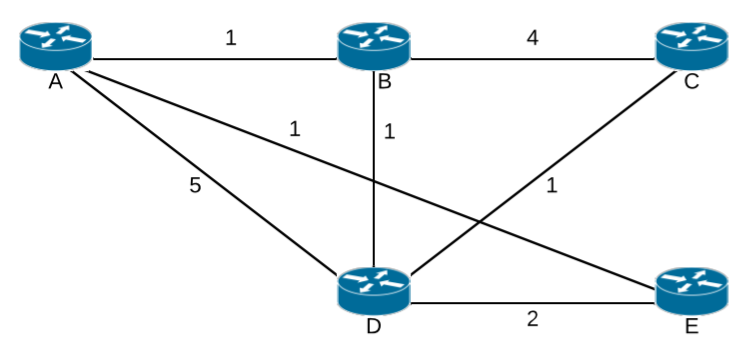
\includegraphics[width=10cm]{esercizio2}
	\end{figure}
	\newline
	Inizializzo le tabelle di routing di ogni nodo inserendo solo i nodi direttamente connessi (per semplicità includo tutte le destinazioni anche se sono ignote, queste avranno costo e NH vuoto).
	\begin{table}[h!]
		\begin{tabular}{|c||c||c|}
 			\hline
	 		\multicolumn{3}{|c|}{A} \\
 			\hline
 			Dst & Cost & NH\\
 			\hline
 			A & 0 & - \\
 			B & 1 & B \\
 			C &   &   \\
 			D & 5 & D \\
 			E & 1 & E \\
 			\hline
		\end{tabular}
		\begin{tabular}{|c||c||c|}
 			\hline
	 		\multicolumn{3}{|c|}{B} \\
 			\hline
 			Dst & Cost & NH\\
 			\hline
 			A & 1 & A \\
 			B & 0 & - \\
 			C & 4 & C  \\
 			D & 1 & D \\
 			E &   &   \\
 			\hline
		\end{tabular}
		\begin{tabular}{|c||c||c|}
 			\hline
	 		\multicolumn{3}{|c|}{C} \\
 			\hline
 			Dst & Cost & NH\\
 			\hline
 			A &   &   \\
 			B & 4 & B \\
 			C & 0 & - \\
 			D & 1 & D \\
 			E &   &   \\
 			\hline
		\end{tabular}
		\begin{tabular}{|c||c||c|}
 			\hline
	 		\multicolumn{3}{|c|}{D} \\
 			\hline
 			Dst & Cost & NH\\
 			\hline
 			A & 5 & A \\
 			B & 1 & B \\
 			C & 1 & C \\
 			D & 0 & - \\
 			E & 2 & E \\
 			\hline
		\end{tabular}
		\begin{tabular}{|c||c||c|}
 			\hline
	 		\multicolumn{3}{|c|}{E} \\
 			\hline
 			Dst & Cost & NH\\
 			\hline
 			A & 1 & A \\
 			B &   &   \\
 			C &   &   \\
 			D & 2 & D \\
 			E & 0 & - \\
 			\hline
		\end{tabular}
	\end{table}
	\newline \newline
	$E$ manda il suo DV: $\{(A,1),(D,2)\}$ a $\{D,A\}$.
	\newline
	$D$ e $A$ scoprono una nuova rotta per raggiungersi con costo inferiore, attraverso $E$.
	\begin{table}[h!]
		\begin{tabular}{|c||c||c|}
 			\hline
	 		\multicolumn{3}{|c|}{A} \\
 			\hline
 			Dst & Cost & NH\\
 			\hline
 			A & 0 & - \\
 			B & 1 & B \\
 			C &   &   \\
 			D & $\color{red} 3$ & $\color{red} E$ \\
 			E & 1 & E \\
 			\hline
		\end{tabular}
		\begin{tabular}{|c||c||c|}
 			\hline
	 		\multicolumn{3}{|c|}{B} \\
 			\hline
 			Dst & Cost & NH\\
 			\hline
 			A & 1 & A \\
 			B & 0 & - \\
 			C & 4 & C  \\
 			D & 1 & D \\
 			E &   &   \\
 			\hline
		\end{tabular}
		\begin{tabular}{|c||c||c|}
 			\hline
	 		\multicolumn{3}{|c|}{C} \\
 			\hline
 			Dst & Cost & NH\\
 			\hline
 			A &   &   \\
 			B & 4 & B \\
 			C & 0 & - \\
 			D & 1 & D \\
 			E &   &   \\
 			\hline
		\end{tabular}
		\begin{tabular}{|c||c||c|}
 			\hline
	 		\multicolumn{3}{|c|}{D} \\
 			\hline
 			Dst & Cost & NH\\
 			\hline
 			A & $\color{red} 3$ & $\color{red} E$ \\
 			B & 1 & B \\
 			C & 1 & C \\
 			D & 0 & - \\
 			E & 2 & E \\
 			\hline
		\end{tabular}
		\begin{tabular}{|c||c||c|}
 			\hline
	 		\multicolumn{3}{|c|}{E} \\
 			\hline
 			Dst & Cost & NH\\
 			\hline
 			A & 1 & A \\
 			B &   &   \\
 			C &   &   \\
 			D & 2 & D \\
 			E & 0 & - \\
 			\hline
		\end{tabular}
	\end{table}
	\newline \newline \newline
	$B$ manda il suo DV: $\{(A,1),(C,4),(D,1)\}$ a $\{A,C,D\}$.
	\newline
	$A$ e $D$ scoprono un nuovo percorso con costo inferiore attraverso $D$.
	\newline
	$A$ viene a conoscenza del nodo $C$ (e viceversa) attraverso il nodo $B$.
	\begin{table}[h!]
		\begin{tabular}{|c||c||c|}
 			\hline
	 		\multicolumn{3}{|c|}{A} \\
 			\hline
 			Dst & Cost & NH\\
 			\hline
 			A & 0 & - \\
 			B & 1 & B \\
 			C & $\color{red} 5$ & $\color{red} B$ \\
 			D & $\color{red} 2$ & $\color{red} B$ \\
 			E & 1 & E \\
 			\hline
		\end{tabular}
		\begin{tabular}{|c||c||c|}
 			\hline
	 		\multicolumn{3}{|c|}{B} \\
 			\hline
 			Dst & Cost & NH\\
 			\hline
 			A & 1 & A \\
 			B & 0 & - \\
 			C & 4 & C  \\
 			D & 1 & D \\
 			E &   &   \\
 			\hline
		\end{tabular}
		\begin{tabular}{|c||c||c|}
 			\hline
	 		\multicolumn{3}{|c|}{C} \\
 			\hline
 			Dst & Cost & NH\\
 			\hline
 			A & $\color{red} 5$ & $\color{red} B$ \\
 			B & 4 & B \\
 			C & 0 & - \\
 			D & 1 & D \\
 			E &   &   \\
 			\hline
		\end{tabular}
		\begin{tabular}{|c||c||c|}
 			\hline
	 		\multicolumn{3}{|c|}{D} \\
 			\hline
 			Dst & Cost & NH\\
 			\hline
 			A & $\color{red} 2$ & $\color{red} B$ \\
 			B & 1 & B \\
 			C & 1 & C \\
 			D & 0 & - \\
 			E & 2 & E \\
 			\hline
		\end{tabular}
		\begin{tabular}{|c||c||c|}
 			\hline
	 		\multicolumn{3}{|c|}{E} \\
 			\hline
 			Dst & Cost & NH\\
 			\hline
 			A & 1 & A \\
 			B &   &   \\
 			C &   &   \\
 			D & 2 & D \\
 			E & 0 & - \\
 			\hline
		\end{tabular}
	\end{table}
	\newline \newline
	$A$ manda il suo DV: $\{(B,1),(C,5),(D,2),(E,1)\}$ a $\{B,D,E\}$.
	\newline
	$B$ viene a conoscenza del nodo $E$ (e viceversa) e del nodo $C$ (ma $C$ ancora non sa che esiste $B$).
	\begin{table}[h!]
		\begin{tabular}{|c||c||c|}
 			\hline
	 		\multicolumn{3}{|c|}{A} \\
 			\hline
 			Dst & Cost & NH\\
 			\hline
 			A & 0 & - \\
 			B & 1 & B \\
 			C & 5 & B \\
 			D & 2 & B \\
 			E & 1 & E \\
 			\hline
		\end{tabular}
		\begin{tabular}{|c||c||c|}
 			\hline
	 		\multicolumn{3}{|c|}{B} \\
 			\hline
 			Dst & Cost & NH\\
 			\hline
 			A & 1 & A \\
 			B & 0 & - \\
 			C & 4 & C  \\
 			D & 1 & D \\
 			E & $\color{red} 2$ & $\color{red} A$ \\
 			\hline
		\end{tabular}
		\begin{tabular}{|c||c||c|}
 			\hline
	 		\multicolumn{3}{|c|}{C} \\
 			\hline
 			Dst & Cost & NH\\
 			\hline
 			A & 5 & B \\
 			B & 4 & B \\
 			C & 0 & - \\
 			D & 1 & D \\
 			E &   &   \\
 			\hline
		\end{tabular}
		\begin{tabular}{|c||c||c|}
 			\hline
	 		\multicolumn{3}{|c|}{D} \\
 			\hline
 			Dst & Cost & NH\\
 			\hline
 			A & 2 & B \\
 			B & 1 & B \\
 			C & 1 & C \\
 			D & 0 & - \\
 			E & 2 & E \\
 			\hline
		\end{tabular}
		\begin{tabular}{|c||c||c|}
 			\hline
	 		\multicolumn{3}{|c|}{E} \\
 			\hline
 			Dst & Cost & NH\\
 			\hline
 			A & 1 & A \\
 			B & $\color{red} 2$ & $\color{red} A$ \\
 			C & $\color{red} 6$ & $\color{red} A$ \\
 			D & 2 & D \\
 			E & 0 & - \\
 			\hline
		\end{tabular}
	\end{table}
	\newline \newline
	$C$ manda il suo DV: $\{(A,5),(B,4),(D,1)\}$ a $\{B,D\}$.
	\newline
	Non ci sono modifiche, non ci sono percorsi migliori ne scoperte di nuovi nodi.
	\begin{table}[h!]
		\begin{tabular}{|c||c||c|}
 			\hline
	 		\multicolumn{3}{|c|}{A} \\
 			\hline
 			Dst & Cost & NH\\
 			\hline
 			A & 0 & - \\
 			B & 1 & B \\
 			C & 5 & B \\
 			D & 2 & B \\
 			E & 1 & E \\
 			\hline
		\end{tabular}
		\begin{tabular}{|c||c||c|}
 			\hline
	 		\multicolumn{3}{|c|}{B} \\
 			\hline
 			Dst & Cost & NH\\
 			\hline
 			A & 1 & A \\
 			B & 0 & - \\
 			C & 4 & C  \\
 			D & 1 & D \\
 			E & 2 & A \\
 			\hline
		\end{tabular}
		\begin{tabular}{|c||c||c|}
 			\hline
	 		\multicolumn{3}{|c|}{C} \\
 			\hline
 			Dst & Cost & NH\\
 			\hline
 			A & 5 & B \\
 			B & 4 & B \\
 			C & 0 & - \\
 			D & 1 & D \\
 			E &   &   \\
 			\hline
		\end{tabular}
		\begin{tabular}{|c||c||c|}
 			\hline
	 		\multicolumn{3}{|c|}{D} \\
 			\hline
 			Dst & Cost & NH\\
 			\hline
 			A & 2 & B \\
 			B & 1 & B \\
 			C & 1 & C \\
 			D & 0 & - \\
 			E & 2 & E \\
 			\hline
		\end{tabular}
		\begin{tabular}{|c||c||c|}
 			\hline
	 		\multicolumn{3}{|c|}{E} \\
 			\hline
 			Dst & Cost & NH\\
 			\hline
 			A & 1 & A \\
 			B & 2 & A \\
 			C & 6 & A \\
 			D & 2 & D \\
 			E & 0 & - \\
 			\hline
		\end{tabular}
	\end{table}
	\newline \newline
	$D$ manda il suo DV: $\{(A,2),(B,1),(C,1),(E,2)\}$ a $\{A,B,C,E\}$.
	\newline
	$B$ scopre un percorso migliore verso $C$ (e viceversa).
	\newline
	$C$ scopre un percorso migliore verso $A$ (ma non viceversa) e scopre anche il nodo $E$.
	\begin{table}[h!]
		\begin{tabular}{|c||c||c|}
 			\hline
	 		\multicolumn{3}{|c|}{A} \\
 			\hline
 			Dst & Cost & NH\\
 			\hline
 			A & 0 & - \\
 			B & 1 & B \\
 			C & 5 & B \\
 			D & 2 & B \\
 			E & 1 & E \\
 			\hline
		\end{tabular}
		\begin{tabular}{|c||c||c|}
 			\hline
	 		\multicolumn{3}{|c|}{B} \\
 			\hline
 			Dst & Cost & NH\\
 			\hline
 			A & 1 & A \\
 			B & 0 & - \\
 			C & $\color{red} 2$ & $\color{red} D$ \\
 			D & 1 & D \\
 			E & 2 & A \\
 			\hline
		\end{tabular}
		\begin{tabular}{|c||c||c|}
 			\hline
	 		\multicolumn{3}{|c|}{C} \\
 			\hline
 			Dst & Cost & NH\\
 			\hline
 			A & $\color{red} 3$ & $\color{red} D$ \\
 			B & $\color{red} 2$ & $\color{red} D$ \\
 			C & 0 & - \\
 			D & 1 & D \\
 			E & $\color{red} 3$ & $\color{red} D$ \\
 			\hline
		\end{tabular}
		\begin{tabular}{|c||c||c|}
 			\hline
	 		\multicolumn{3}{|c|}{D} \\
 			\hline
 			Dst & Cost & NH\\
 			\hline
 			A & 2 & B \\
 			B & 1 & B \\
 			C & 1 & C \\
 			D & 0 & - \\
 			E & 2 & E \\
 			\hline
		\end{tabular}
		\begin{tabular}{|c||c||c|}
 			\hline
	 		\multicolumn{3}{|c|}{E} \\
 			\hline
 			Dst & Cost & NH\\
 			\hline
 			A & 1 & A \\
 			B & 2 & A \\
 			C & $\color{red} 3$ & $\color{red} D$ \\
 			D & 2 & D \\
 			E & 0 & - \\
 			\hline
		\end{tabular}
	\end{table}
	\newline \newline
	\textbf{E' stato inviato il set completo di messaggi tra i router, ma non abbiamo raggiunto la convergenza; il nodo $A$ deve ancora scoprire il percorso migliore verso $C$.}
	\newline \newline \newline
	$E$ manda il suo DV: $\{(A,1),(B,2),(C,3),(D,2)\}$ a $\{A,D\}$.
	\newline
	$A$ scopre un nuovo percorso verso $C$ con costo inferiore attraverso $E$.
	\begin{table}[h!]
		\begin{tabular}{|c||c||c|}
 			\hline
	 		\multicolumn{3}{|c|}{A} \\
 			\hline
 			Dst & Cost & NH\\
 			\hline
 			A & 0 & - \\
 			B & 1 & B \\
 			C & $\color{red} 4$ & $\color{red} E$ \\
 			D & 2 & B \\
 			E & 1 & E \\
 			\hline
		\end{tabular}
		\begin{tabular}{|c||c||c|}
 			\hline
	 		\multicolumn{3}{|c|}{B} \\
 			\hline
 			Dst & Cost & NH\\
 			\hline
 			A & 1 & A \\
 			B & 0 & - \\
 			C & 2 & D \\
 			D & 1 & D \\
 			E & 2 & A \\
 			\hline
		\end{tabular}
		\begin{tabular}{|c||c||c|}
 			\hline
	 		\multicolumn{3}{|c|}{C} \\
 			\hline
 			Dst & Cost & NH\\
 			\hline
 			A & 3 & D \\
 			B &3 & D \\
 			C & 0 & - \\
 			D & 1 & D \\
 			E & 3 & D \\
 			\hline
		\end{tabular}
		\begin{tabular}{|c||c||c|}
 			\hline
	 		\multicolumn{3}{|c|}{D} \\
 			\hline
 			Dst & Cost & NH\\
 			\hline
 			A & 2 & B \\
 			B & 1 & B \\
 			C & 1 & C \\
 			D & 0 & - \\
 			E & 2 & E \\
 			\hline
		\end{tabular}
		\begin{tabular}{|c||c||c|}
 			\hline
	 		\multicolumn{3}{|c|}{E} \\
 			\hline
 			Dst & Cost & NH\\
 			\hline
 			A & 1 & A \\
 			B & 2 & A \\
 			C & 3 & D \\
 			D & 2 & D \\
 			E & 0 & - \\
 			\hline
		\end{tabular}
	\end{table}
	\newline \newline
	E' stato inviato il set completo di messaggi tra i router, ma non abbiamo raggiunto la convergenza; il nodo $A$ deve ancora scoprire il percorso migliore verso $C$.
	\newline \newline
	$B$ manda il suo DV: $\{(A,1),(C,2),(D,1),(E,2)\}$ a $\{A,D\}$.
	\newline
	$A$ finalmente scopre il percorso migliore verso $C$ attraverso $B$, e così facendo raggiungiamo la convergenza.
	\begin{table}[h!]
		\begin{tabular}{|c||c||c|}
 			\hline
	 		\multicolumn{3}{|c|}{A} \\
 			\hline
 			Dst & Cost & NH\\
 			\hline
 			A & 0 & - \\
 			B & 1 & B \\
 			C & $\color{red} 3$ & $\color{red} B$ \\
 			D & 2 & B \\
 			E & 1 & E \\
 			\hline
		\end{tabular}
		\begin{tabular}{|c||c||c|}
 			\hline
	 		\multicolumn{3}{|c|}{B} \\
 			\hline
 			Dst & Cost & NH\\
 			\hline
 			A & 1 & A \\
 			B & 0 & - \\
 			C & 2 & D \\
 			D & 1 & D \\
 			E & 2 & A \\
 			\hline
		\end{tabular}
		\begin{tabular}{|c||c||c|}
 			\hline
	 		\multicolumn{3}{|c|}{C} \\
 			\hline
 			Dst & Cost & NH\\
 			\hline
 			A & 3 & D \\
 			B &3 & D \\
 			C & 0 & - \\
 			D & 1 & D \\
 			E & 3 & D \\
 			\hline
		\end{tabular}
		\begin{tabular}{|c||c||c|}
 			\hline
	 		\multicolumn{3}{|c|}{D} \\
 			\hline
 			Dst & Cost & NH\\
 			\hline
 			A & 2 & B \\
 			B & 1 & B \\
 			C & 1 & C \\
 			D & 0 & - \\
 			E & 2 & E \\
 			\hline
		\end{tabular}
		\begin{tabular}{|c||c||c|}
 			\hline
	 		\multicolumn{3}{|c|}{E} \\
 			\hline
 			Dst & Cost & NH\\
 			\hline
 			A & 1 & A \\
 			B & 2 & A \\
 			C & 3 & D \\
 			D & 2 & D \\
 			E & 0 & - \\
 			\hline
		\end{tabular}
	\end{table}
	\subsection{Esercizio 3}
	Usando l'algoritmo di routing di tipo Distance-vector, mostrare l'evoluzione delle tabelle di routing per ogni nodo, considerando che i DV vengono inoltrati dai router seguendo l'ordine: ${E,D,C,B,A}$.
	\begin{figure}[h!]
	\centering
	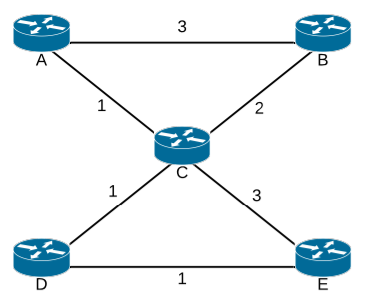
\includegraphics[width=9cm]{esercizio3}
	\end{figure}
	\newline
	Inizializzo le tabelle di routing di ogni nodo inserendo solo i nodi direttamente connessi (per semplicità includo tutte le destinazioni anche se sono ignote, queste avranno costo e NH vuoto).
	\begin{table}[h!]
		\begin{tabular}{|c||c||c|}
 			\hline
	 		\multicolumn{3}{|c|}{A} \\
 			\hline
 			Dst & Cost & NH\\
 			\hline
 			A & 0 & - \\
 			B & 3 & B \\
 			C & 1 & C \\
 			D &   &   \\
 			E &   &   \\
 			\hline
		\end{tabular}
		\begin{tabular}{|c||c||c|}
 			\hline
	 		\multicolumn{3}{|c|}{B} \\
 			\hline
 			Dst & Cost & NH\\
 			\hline
 			A & 3 & A \\
 			B & 0 & - \\
 			C & 2 & C  \\
 			D &   &   \\
 			E &   &   \\
 			\hline
		\end{tabular}
		\begin{tabular}{|c||c||c|}
 			\hline
	 		\multicolumn{3}{|c|}{C} \\
 			\hline
 			Dst & Cost & NH\\
 			\hline
 			A & 1 & A \\
 			B & 2 & B \\
 			C & 0 & - \\
 			D & 1 & D \\
 			E & 3 & C \\
 			\hline
		\end{tabular}
		\begin{tabular}{|c||c||c|}
 			\hline
	 		\multicolumn{3}{|c|}{D} \\
 			\hline
 			Dst & Cost & NH\\
 			\hline
 			A &   &   \\
 			B &   &   \\
 			C & 1 & C \\
 			D & 0 & - \\
 			E & 1 & E \\
 			\hline
		\end{tabular}
		\begin{tabular}{|c||c||c|}
 			\hline
	 		\multicolumn{3}{|c|}{E} \\
 			\hline
 			Dst & Cost & NH\\
 			\hline
 			A &   &   \\
 			B &   &   \\
 			C & 3 & C \\
 			D & 1 & D \\
 			E & 0 & - \\
 			\hline
		\end{tabular}
	\end{table}
	\newline \newline \newline 
	$E$ manda il suo DV: $\{(C,3),(D,1)\}$ a $\{D,C\}$.
	\newline
	Nulla cambia, non ci sono tratte migliori ne scoperta di nuovi nodi.
	\begin{table}[h!]
		\begin{tabular}{|c||c||c|}
 			\hline
	 		\multicolumn{3}{|c|}{A} \\
 			\hline
 			Dst & Cost & NH\\
 			\hline
 			A & 0 & - \\
 			B & 3 & B \\
 			C & 1 & C \\
 			D &   &   \\
 			E &   &   \\
 			\hline
		\end{tabular}
		\begin{tabular}{|c||c||c|}
 			\hline
	 		\multicolumn{3}{|c|}{B} \\
 			\hline
 			Dst & Cost & NH\\
 			\hline
 			A & 3 & A \\
 			B & 0 & - \\
 			C & 2 & C  \\
 			D &   &   \\
 			E &   &   \\
 			\hline
		\end{tabular}
		\begin{tabular}{|c||c||c|}
 			\hline
	 		\multicolumn{3}{|c|}{C} \\
 			\hline
 			Dst & Cost & NH\\
 			\hline
 			A & 1 & A \\
 			B & 2 & B \\
 			C & 0 & - \\
 			D & 1 & D \\
 			E & 3 & C \\
 			\hline
		\end{tabular}
		\begin{tabular}{|c||c||c|}
 			\hline
	 		\multicolumn{3}{|c|}{D} \\
 			\hline
 			Dst & Cost & NH\\
 			\hline
 			A &   &   \\
 			B &   &   \\
 			C & 1 & C \\
 			D & 0 & - \\
 			E & 1 & E \\
 			\hline
		\end{tabular}
		\begin{tabular}{|c||c||c|}
 			\hline
	 		\multicolumn{3}{|c|}{E} \\
 			\hline
 			Dst & Cost & NH\\
 			\hline
 			A &   &   \\
 			B &   &   \\
 			C & 3 & C \\
 			D & 1 & D \\
 			E & 0 & - \\
 			\hline
		\end{tabular}
	\end{table}
	\newline \newline
	$D$ manda il suo DV: $\{(C,1),(E,1)\}$ a $\{C,E\}$.
	\newline
	$E$ scopre un nuovo percorso verso $C$ (e viceversa) con costo inferiore attraverso $D$.
	\begin{table}[h!]
		\begin{tabular}{|c||c||c|}
 			\hline
	 		\multicolumn{3}{|c|}{A} \\
 			\hline
 			Dst & Cost & NH\\
 			\hline
 			A & 0 & - \\
 			B & 3 & B \\
 			C & 1 & C \\
 			D &   &   \\
 			E &   &   \\
 			\hline
		\end{tabular}
		\begin{tabular}{|c||c||c|}
 			\hline
	 		\multicolumn{3}{|c|}{B} \\
 			\hline
 			Dst & Cost & NH\\
 			\hline
 			A & 3 & A \\
 			B & 0 & - \\
 			C & 2 & C  \\
 			D &   &   \\
 			E &   &   \\
 			\hline
		\end{tabular}
		\begin{tabular}{|c||c||c|}
 			\hline
	 		\multicolumn{3}{|c|}{C} \\
 			\hline
 			Dst & Cost & NH\\
 			\hline
 			A & 1 & A \\
 			B & 2 & B \\
 			C & 0 & - \\
 			D & 1 & D \\
 			E & $\color{red} 2$ & $\color{red} D$ \\
 			\hline
		\end{tabular}
		\begin{tabular}{|c||c||c|}
 			\hline
	 		\multicolumn{3}{|c|}{D} \\
 			\hline
 			Dst & Cost & NH\\
 			\hline
 			A &   &   \\
 			B &   &   \\
 			C & 1 & C \\
 			D & 0 & - \\
 			E & 1 & E \\
 			\hline
		\end{tabular}
		\begin{tabular}{|c||c||c|}
 			\hline
	 		\multicolumn{3}{|c|}{E} \\
 			\hline
 			Dst & Cost & NH\\
 			\hline
 			A &   &   \\
 			B &   &   \\
 			C & $\color{red} 2$ & $\color{red} D$ \\
 			D & 1 & D \\
 			E & 0 & - \\
 			\hline
		\end{tabular}
	\end{table}
	\newline \newline
	$C$ manda il suo DV: $\{(A,1),(B,2),(D,1),(E,2)\}$ a $\{C,E\}$.
	\newline
	$A$ e $B$ vengono a conoscenza dei nodi $D$ e $D$ (e viceversa).
	\begin{table}[h!]
		\begin{tabular}{|c||c||c|}
 			\hline
	 		\multicolumn{3}{|c|}{A} \\
 			\hline
 			Dst & Cost & NH\\
 			\hline
 			A & 0 & - \\
 			B & 3 & B \\
 			C & 1 & C \\
 			D & $\color{red} 2$ & $\color{red} C$ \\
 			E & $\color{red} 3$ & $\color{red} C$ \\
 			\hline
		\end{tabular}
		\begin{tabular}{|c||c||c|}
 			\hline
	 		\multicolumn{3}{|c|}{B} \\
 			\hline
 			Dst & Cost & NH\\
 			\hline
 			A & 3 & A \\
 			B & 0 & - \\
 			C & 2 & C  \\
 			D & $\color{red} 3$ & $\color{red} C$ \\
 			E & $\color{red} 4$ & $\color{red} C$ \\
 			\hline
		\end{tabular}
		\begin{tabular}{|c||c||c|}
 			\hline
	 		\multicolumn{3}{|c|}{C} \\
 			\hline
 			Dst & Cost & NH\\
 			\hline
 			A & 1 & A \\
 			B & 2 & B \\
 			C & 0 & - \\
 			D & 1 & D \\
 			E & 2 & D \\
 			\hline
		\end{tabular}
		\begin{tabular}{|c||c||c|}
 			\hline
	 		\multicolumn{3}{|c|}{D} \\
 			\hline
 			Dst & Cost & NH\\
 			\hline
 			A & $\color{red} 2$ & $\color{red} C$ \\
 			B & $\color{red} 3$ & $\color{red} C$ \\
 			C & 1 & C \\
 			D & 0 & - \\
 			E & 1 & E \\
 			\hline
		\end{tabular}
		\begin{tabular}{|c||c||c|}
 			\hline
	 		\multicolumn{3}{|c|}{E} \\
 			\hline
 			Dst & Cost & NH\\
 			\hline
 			A & $\color{red} 4$ & $\color{red} C$ \\
 			B & $\color{red} 5$ & $\color{red} C$ \\
 			C & 2 & D \\
 			D & 1 & D \\
 			E & 0 & - \\
 			\hline
		\end{tabular}
	\end{table}
	\newline \newline
	I nodi $B$ e $A$ mandano i loro DV a $\{A,B,C\}$ ma non ci sono modifiche. Il set di messaggi è finito, ma non abbiamo ancora raggiunto la convergenza, infatti il nodo E deve ancora trovare il percorso migliore verso i nodi A e B.
	\newline \newline $E$ manda il suo Dv ai nodi $\{D,C\}$ ma nulla cambia.
	\newline Quando il nodo $D$ manda il suo DV ai nodi $\{C,E\}$, $E$ trova un percorso migliore verso i nodi $\{A,B\}$ attraverso $D$; la tabella di $E$ viene modificata nel seguente modo:
	\begin{itemize}
		\item $A$ - $\color{red} 3$ $\color{red} D$
		\item $B$ - $\color{red} 4$ $\color{red} D$
	\end{itemize}
	\end{document}
